\documentclass[11pt]{article}

\usepackage[margin=1in]{geometry}
\usepackage{graphicx}
\usepackage{booktabs}
\usepackage{xcolor}
\usepackage{listings}
\usepackage{amsmath}
\usepackage{caption}
\usepackage{float}
\usepackage[hidelinks]{hyperref}
\usepackage{fancyhdr}
\usepackage{enumitem}
\usepackage{titlesec}

\definecolor{amdred}{HTML}{ED1C24}
\definecolor{codebg}{HTML}{F5F5F7}
\definecolor{codekw}{HTML}{0A7D8C}
\definecolor{codecmt}{HTML}{6A737D}
\definecolor{rulegray}{HTML}{D4D4D8}

\hypersetup{colorlinks=true, linkcolor=amdred, urlcolor=amdred, citecolor=amdred}

\titleformat{\section}{\Large\bfseries\color{amdred}}{\thesection}{0.6em}{}
\titleformat{\subsection}{\large\bfseries}{\thesubsection}{0.6em}{}

\pagestyle{fancy}
\fancyhf{}
\lhead{\textcolor{amdred}{\textbf{AMD AI4Science Studio}}}
\rhead{HydraGNN Training \& Inference Guide}
\cfoot{\thepage}
\renewcommand{\headrulewidth}{0.4pt}

\lstdefinestyle{sh}{
  backgroundcolor=\color{codebg}, basicstyle=\ttfamily\footnotesize,
  keywordstyle=\color{codekw}\bfseries, commentstyle=\color{codecmt}\itshape,
  breaklines=true, frame=single, rulecolor=\color{rulegray},
  columns=fullflexible, showstringspaces=false, xleftmargin=6pt, xrightmargin=6pt,
  aboveskip=8pt, belowskip=8pt,
}
\lstset{style=sh}

\newcommand{\code}[1]{\colorbox{codebg}{\texttt{\small #1}}}

\begin{document}

% ── Cover ────────────────────────────────────────────────────────────────
\begin{titlepage}
\centering
\vspace*{2.5cm}
{\Huge\bfseries\color{amdred} AMD AI4Science Studio\par}
\vspace{0.6cm}
{\LARGE\bfseries HydraGNN: Training \& Inference Guide\par}
\vspace{0.4cm}
{\large Materials energy prediction on Alexandria DFT data,\\ trained and served on AMD Instinct\texttrademark{} MI355X GPUs\par}
\vspace{2cm}
\begin{minipage}{0.85\textwidth}
\centering\itshape
A hands-on reference for the HydraGNN demo: environment preparation, multi-GPU
training, single-structure inference, the four curated demonstration materials,
the 1-GPU vs 8-GPU scaling study, and the studio walkthrough. All numbers are
real, produced by the studio's SLURM pipeline; nothing in this document is
synthetic.
\end{minipage}
\vfill
{\large Author: Sreekanth Pannala\par}
\vspace{0.3cm}
{\small Generated \today\par}
\end{titlepage}

\tableofcontents
\newpage

% ── 1. Overview ──────────────────────────────────────────────────────────
\section{Overview}

HydraGNN is a graph neural network for atomistic property prediction developed at
Oak Ridge National Laboratory~\cite{hydragnn,lupomercado2022}. In the AI4Science
Studio it predicts the DFT per-atom energy of inorganic crystals drawn from the
Alexandria database~\cite{alexandria,schmidt2023}. This guide documents the full
workflow behind the demo:

\begin{itemize}[nosep]
  \item \textbf{Preparation} --- container, overlay, dataset, and cluster setup.
  \item \textbf{Training} --- the 8-GPU DDP production run (v3) and a matched
        1-GPU run used for the scaling study.
  \item \textbf{Inference} --- single-structure energy prediction that live mode
        and demo mode share bit-for-bit.
  \item \textbf{Results} --- the four curated demonstration materials, the
        scaling comparison, and a MACE foundation-model sanity check.
  \item \textbf{Demo script} --- how the studio wizard drives the workflow.
\end{itemize}

\begin{figure}[H]
\centering
\includegraphics[width=0.92\textwidth]{../images/hydragnn-overview.png}
\caption{HydraGNN maps a periodic crystal to a graph (atoms as nodes, bonds as
edges) and predicts the per-atom formation energy. The model used here is a
Principal Neighbourhood Aggregation (PNA) message-passing network~\cite{pna}.}
\end{figure}

\subsection{The prediction target}

Each structure carries a DFT-computed per-atom energy $E_{\text{DFT}}$ (eV/atom)
in the Alexandria formation-energy reference. HydraGNN predicts
$\hat{E}$, and we report the absolute error $|\hat{E}-E_{\text{DFT}}|$. Accuracy
over the held-out set is summarized by Pearson correlation, coefficient of
determination $R^2$, and mean absolute error (MAE).

% ── 2. Environment preparation ───────────────────────────────────────────
\section{Environment Preparation}

All heavy compute runs \emph{inside an Apptainer container on a compute node}.
The login node has no GPU and no scientific Python stack; those live in the
container overlay.

\subsection{Fixed components}

\begin{table}[H]
\centering\small
\begin{tabular}{@{}ll@{}}
\toprule
\textbf{Component} & \textbf{Path / value} \\
\midrule
Cluster & LUX (AMD Instinct MI355X, 8 GPU/node) \\
Container (SIF) & \texttt{pytorch\_rocm7.2.2\_ubuntu24.04\_py3.12\_...\_2.10.0.sif} \\
Overlay (HydraGNN + adios2) & \texttt{overlays/hydragnn-overlay.img} \\
Framework & PyTorch 2.10 (ROCm 7.2.2), HydraGNN (PNA) \\
Dataset & Alexandria-v2 (ADIOS2 \texttt{.bp}), 268{,}227 val structures \\
Work root & \texttt{\$AI4S\_SHARED\_DIR/models/HydraGNN/train\_work} \\
\bottomrule
\end{tabular}
\caption{Fixed environment. The dataset ships precomputed periodic-boundary (PBC)
graph edges, which the model consumes directly.}
\end{table}

\subsection{In-container environment}

Every job activates the container venv and sets the ROCm/adios2 paths:

\begin{lstlisting}[language=bash]
source /opt/venv/bin/activate
export HSA_NO_SCRATCH_RECLAIM=1
export PYTHONPATH=$HG_INFER_REPO:/opt/hydragnn-pkgs
export LD_LIBRARY_PATH=/opt/hydragnn-pkgs/adios2:/opt/venv/lib/python3.12/site-packages/torch/lib
\end{lstlisting}

\subsection{Multi-GPU launch notes (hard-won)}

\begin{itemize}[nosep]
  \item On MI355X, \textbf{all 8 GPUs must remain visible to every rank} so RCCL
        can read the full XGMI topology; the per-rank device is chosen from
        \texttt{SLURM\_LOCALID}. Never set \texttt{ROCR\_VISIBLE\_DEVICES} per rank.
  \item Strip \texttt{PMIX\_/PMI\_/OMPI\_} environment variables before
        \code{apptainer}, else \code{MPI\_Init} aborts on a null communicator.
  \item Use \code{srun --mpi=pmix --cpu-bind=none --gpus-per-node=8}.
  \item Compute nodes are air-gapped (no DNS). Anything requiring the network
        (pip, model downloads) must be staged on the login node first.
\end{itemize}

% ── 3. Dataset ───────────────────────────────────────────────────────────
\section{Dataset: Alexandria DFT}

The Alexandria database~\cite{alexandria,schmidt2023} contains millions of
DFT-relaxed inorganic crystals (PBE functional). The studio uses a preprocessed
ADIOS2 snapshot exposing, per structure: atomic numbers $Z$, Cartesian positions,
the lattice cell, periodic-boundary flags, precomputed graph edges with
interatomic distances, and the DFT energy. Training oversamples three demo-relevant
chemistries (Fe--C, Li--Mn--O, W--Re) so the model is competent on the materials
the demo highlights, while retaining a broad general sample.

% ── 4. Training ──────────────────────────────────────────────────────────
\section{Training}

\subsection{Model and hyperparameters}

\begin{table}[H]
\centering\small
\begin{tabular}{@{}ll@{}}
\toprule
\textbf{Setting} & \textbf{Value} \\
\midrule
Architecture & PNA (Principal Neighbourhood Aggregation)~\cite{pna} \\
Node features & $[Z, x, y, z]$ (atomic number + Cartesian coordinates) \\
Edge features & interatomic distance (\texttt{lengths}) \\
Graph & dataset's stored PBC edges; radius 5.0\,\AA{}, max 20 neighbours \\
Hidden dim / conv layers & 128 / 5 \\
Output head & graph-level energy (shared 2$\times$128, head 128/64/32) \\
Optimizer & AdamW, lr $10^{-3}$, ReduceLROnPlateau \\
Loss / batch / epochs & MSE / 64 / 200 \\
Train split & 80\% (10\% val, 10\% test) \\
\bottomrule
\end{tabular}
\caption{Production (v3) configuration, shared by both scaling runs.}
\end{table}

\subsection{Two runs, one pipeline}

The scaling study compares two runs that differ \emph{only} in data scale and GPU
count. Both use the identical PBC-edge featurizer and the configuration above, so
the comparison isolates the effect of scale.

\begin{table}[H]
\centering\small
\begin{tabular}{@{}lccccc@{}}
\toprule
\textbf{Run} & \textbf{GPUs} & \textbf{Structures} & \textbf{Corr} & \textbf{$R^2$} & \textbf{MAE (eV/atom)} \\
\midrule
1-GPU & 1 & 40{,}000  & 0.8208 & 0.6726 & 0.2882 \\
8-GPU (v3) & 8 & 600{,}000 & \textbf{0.8894} & \textbf{0.7892} & \textbf{0.2395} \\
\bottomrule
\end{tabular}
\caption{Final held-out test metrics. Scaling to 8 GPUs trains on 15$\times$ more
data in comparable wall-clock and improves every metric.}
\end{table}

\subsection{Submitting a run}

The 8-GPU production run is a single \code{sbatch}:

\begin{lstlisting}[language=bash]
cd "$AI4S_SHARED_DIR/models/HydraGNN/train_work"
sbatch scripts/hg_ddp8_v3.sbatch     # 600k structures, 8 GPUs, ~9 min
# 1-GPU matched run (same pipeline, 40k structures):
sbatch scripts/hg_train1_pbc.sbatch
\end{lstlisting}

Each rank runs one container bound to its local GPU; DDP is initialized over NCCL
with a localhost master. The script writes a validation JSON (predictions +
metrics) and the model checkpoint (\texttt{hg\_model\_ddp\_v3.pk}).

\subsection{Convergence and accuracy}

\begin{figure}[H]
\centering
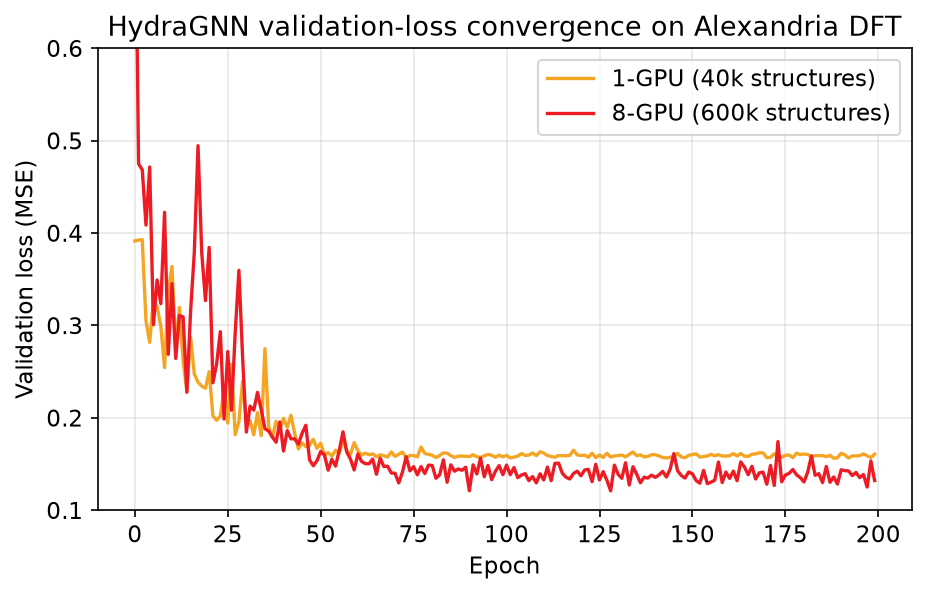
\includegraphics[width=0.8\textwidth]{figs/fig_convergence.png}
\caption{Validation-loss convergence. The 8-GPU run (600k structures) reaches a
lower plateau; the 1-GPU run (40k) shows a mild train/val gap characteristic of a
smaller dataset. Both use the same optimizer schedule.}
\end{figure}

\begin{figure}[H]
\centering
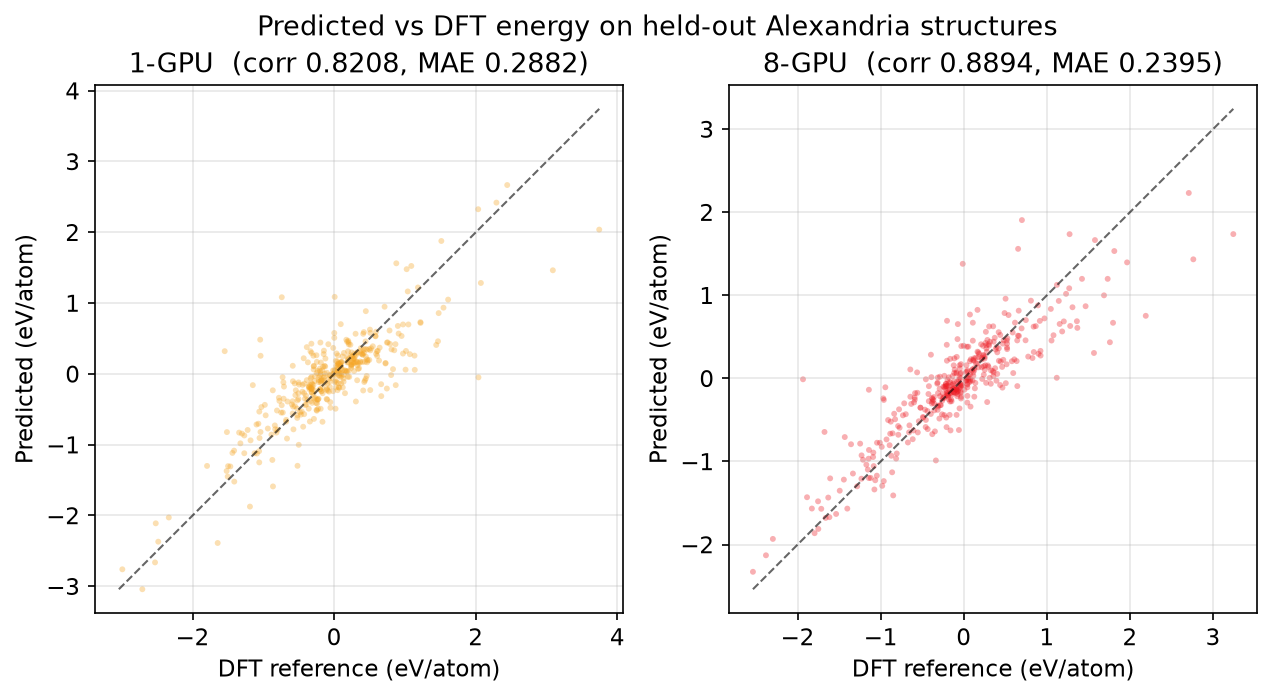
\includegraphics[width=\textwidth]{figs/fig_parity.png}
\caption{Predicted vs DFT energy on held-out structures. Tighter clustering about
the diagonal for the 8-GPU model reflects its higher correlation (0.89 vs 0.82).}
\end{figure}

\begin{figure}[H]
\centering
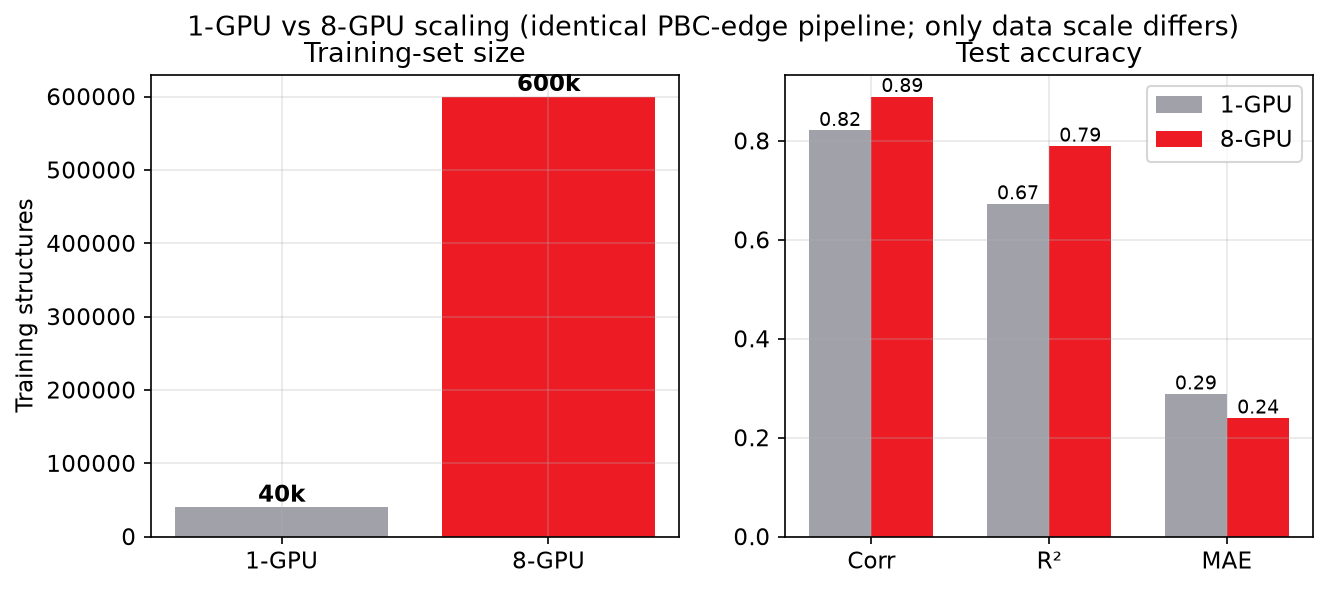
\includegraphics[width=\textwidth]{figs/fig_scaling.png}
\caption{Scaling summary: 15$\times$ more training data (left) yields consistent
accuracy gains across correlation, $R^2$, and MAE (right).}
\end{figure}

\subsection{A note on later epochs}

Validation loss can rise or wander in late epochs. A widening train/val gap
indicates mild overfitting (more pronounced in the 1-GPU run); erratic jumps are
measurement noise on a finite validation set or transient learning-rate effects
before the scheduler intervenes. For the demo the final-epoch checkpoint is used;
a best-epoch (early-stopping) checkpoint is the stricter choice for production.

% ── 5. Inference ─────────────────────────────────────────────────────────
\section{Inference}

Inference featurizes one held-out structure with the \emph{same} PBC-edge graph
used in training, runs the PNA forward pass, and reports predicted vs DFT energy
plus atomic coordinates for the 3D viewer. The featurizer derives its node-feature
width from the checkpoint, so live inference reproduces the trained model exactly.

\begin{lstlisting}[language=bash]
# Single-structure inference (index 2816 = pyrite FeS2)
export MODEL_PATH=.../results/hg_model_ddp_v3.pk
export HG_USE_PBC_EDGES=1 STRUCT_INDEX=2816
export MATERIAL_LABELS_FILE=.../inference/demo_material_labels.json
python3 studio_infer.py    # writes a result JSON the studio harvests
\end{lstlisting}

\paragraph{Live equals demo.} The baked demo predictions and live inference were
verified to match bit-for-bit (energy, formula, and material labels) for all four
curated materials on both the 1-GPU and 8-GPU checkpoints. Demo mode simply
replays a precomputed real inference so the booth needs no GPU wait; live mode runs
the same code on the cluster.

% ── 6. Results: the four demonstration materials ─────────────────────────
\section{Results: Four Real, Practical Materials}

The demo showcases four small, recognizable materials with real experimental
relevance --- not cherry-picked zero-error cases.

\begin{table}[H]
\centering\small
\begin{tabular}{@{}lllcc@{}}
\toprule
\textbf{Material} & \textbf{Formula} & \textbf{Application} & \textbf{8-GPU pred} & \textbf{DFT} \\
\midrule
Pyrite (``fool's gold'') & FeS$_2$   & PV absorber; Li/Na cathode        & $-0.062$ & $-0.056$ \\
Awaruite / permalloy     & FeNi$_3$  & Soft magnet (transformers)        & $-0.026$ & $-0.021$ \\
Sodium ferrite           & NaFeO$_2$ & Na-ion battery cathode            & $-0.892$ & $-0.920$ \\
Iron hydride (design)    & Fe$_2$H$_6$ & H storage / superhydrides       & $+0.155$ & $+0.159$ \\
\bottomrule
\end{tabular}
\caption{Curated demonstration materials (energies in eV/atom). Pyrite, permalloy,
and sodium ferrite are well-characterized experimentally~\cite{pyrite,permalloy,nafeo2};
Fe$_2$H$_6$ is a hypothetical \emph{design candidate} illustrating stability
prediction before synthesis~\cite{superhydride}.}
\end{table}

\begin{figure}[H]
\centering
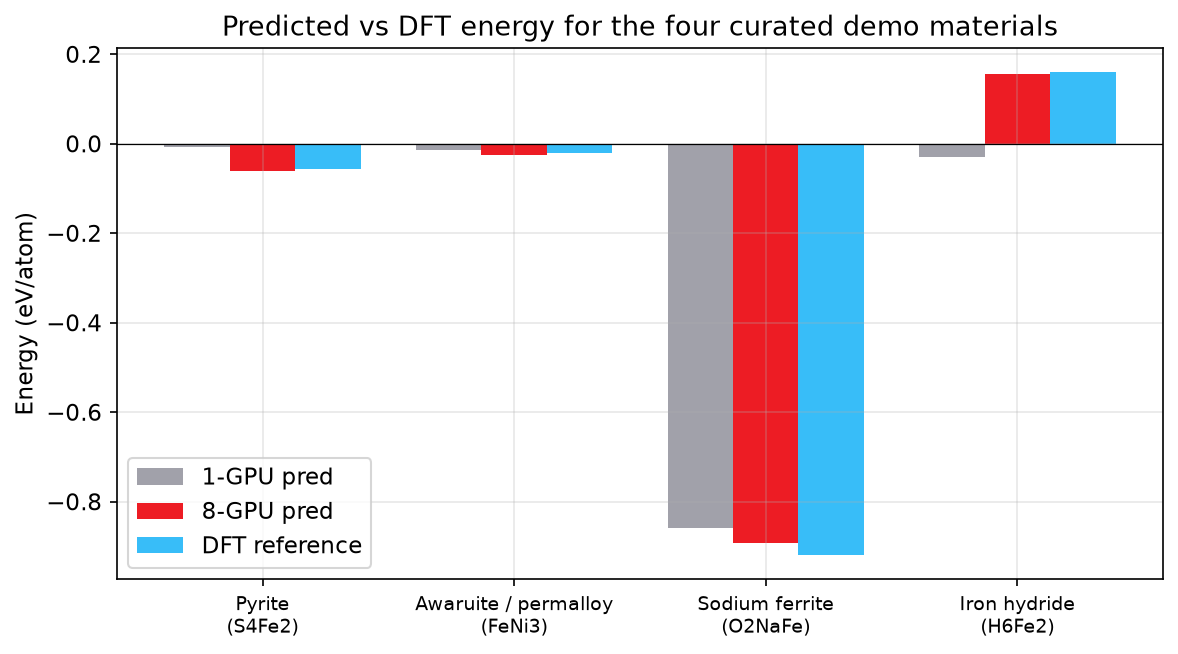
\includegraphics[width=\textwidth]{figs/fig_materials.png}
\caption{Predicted vs DFT energy for the four materials. The 8-GPU model (red)
tracks the DFT reference (blue) closely across chemistries. For the Fe$_2$H$_6$
design candidate the 1-GPU model (grey) even predicts the wrong sign, while the
8-GPU model is essentially correct --- a concrete illustration of why scale
matters for materials discovery.}
\end{figure}

\subsection{Foundation-model sanity check (MACE)}

As a context check we ran MACE-MP-0~\cite{mace,macemp} --- a large equivariant
foundation model --- on the same four structures. MACE-MP-0 reports absolute
energies in the MPtrj/PBE+U reference ($\sim -5$ eV/atom), whereas Alexandria uses
a formation-energy reference ($\sim -0.1$ eV/atom). The two are therefore
\emph{not} on the same numerical scale and cannot be compared directly; the check
confirms our energies are consistent with the Alexandria reference and marks where
a general-purpose foundation model would sit. Meaningfully beating the PNA model's
$\sim$0.24 eV/atom MAE would require an equivariant architecture or angular edge
features, not a configuration tweak.

% ── 7. The studio walkthrough ────────────────────────────────────────────
\section{The Studio Demo Walkthrough}

The AI4Science Studio wraps this pipeline in a five-step wizard (Domain $\to$ Model
$\to$ Configure $\to$ Run $\to$ Analyze). It offers a \textbf{Demo} mode (instant
replay of real precomputed results, no GPU) and a \textbf{Live} mode (submits a
real SLURM job). The screenshots below are from the current build.

\newcommand{\shotpage}[3]{%
\begin{figure}[H]\centering
\setlength{\fboxsep}{0pt}\setlength{\fboxrule}{0.4pt}%
\fbox{\includegraphics[width=0.95\textwidth]{shots/#1}}
\caption{#2 \textit{#3}}\end{figure}}

\shotpage{00_domains.png}{Step 1 --- Choose a scientific domain.}
{HydraGNN lives under Material Science.}

\shotpage{01_models.png}{Step 2 --- Select the model.}
{HydraGNN, the graph foundation model for atomistic energy prediction.}

\shotpage{02_configure_train.png}{Step 3 --- Configure the training-scaling demo.}
{The task toggle selects a 1-GPU vs 8-GPU comparison on real Alexandria DFT data.}

\shotpage{03_run_train.png}{Step 4 --- Run.}
{Demo mode replays the real training result instantly; Live mode submits a SLURM job.}

\shotpage{04_analyze_convergence.png}{Step 5 --- Analyze: scaling study.}
{Real loss curves, training-set size, an 8-GPU parity plot, and the final-metrics table.}

\shotpage{05_configure_infer.png}{Step 3 (Inference) --- Choose the trained checkpoint.}
{The 8-GPU or 1-GPU model is run on a real held-out Alexandria structure.}

\shotpage{06_energy_fes2.png}{Inference --- Pyrite, FeS$_2$.}
{Interactive 3D structure with predicted vs DFT energy and model validation stats.}

\shotpage{07_energy_feni3.png}{Inference --- Awaruite / permalloy, FeNi$_3$.}
{A soft ferromagnetic alloy used in transformer cores and magnetic shielding.}

\shotpage{08_energy_nafeo2.png}{Inference --- Sodium ferrite, NaFeO$_2$.}
{A low-cost sodium-ion battery cathode candidate.}

\shotpage{09_energy_fe2h6.png}{Inference --- Iron hydride, Fe$_2$H$_6$ (design candidate).}
{Predicting the stability of a hypothetical compound before it is synthesized.}

% ── 8. Reproduce ─────────────────────────────────────────────────────────
\section{Reproducing This Guide}

\begin{lstlisting}[language=bash]
# 1. Train (compute node, real GPUs)
sbatch scripts/hg_ddp8_v3.sbatch          # 8-GPU production model (v3)
sbatch scripts/hg_train1_pbc.sbatch       # 1-GPU matched model

# 2. Bake demo predictions on the 4 curated materials
#    (STRUCT_INDICES=2816,3372,29321,1349 ; PBC edges ; labels file)
bash scripts/bake_run.sh                  # via srun in-container

# 3. Regenerate figures and screenshots
python make_figs.py                       # figures from the result JSONs
sbatch docs/hydragnn_guide/capture.slurm  # UI screenshots (Playwright)

# 4. Build this PDF
latexmk -pdf hydragnn_guide.tex
\end{lstlisting}

\begin{thebibliography}{9}
\small
\bibitem{hydragnn} ORNL, \emph{HydraGNN: Distributed PyTorch library for
graph neural networks}. \url{https://github.com/ORNL/HydraGNN}.
\bibitem{lupomercado2022} M. Lupo Pasini \emph{et al.}, ``Scalable training of
graph convolutional neural networks for fast and accurate predictions of
HOMO-LUMO gap,'' \emph{J.\ Cheminform.} \textbf{14}, 55 (2022).
\bibitem{pna} G. Corso \emph{et al.}, ``Principal Neighbourhood Aggregation for
Graph Nets,'' \emph{NeurIPS} (2020). arXiv:2004.05718.
\bibitem{alexandria} J. Schmidt \emph{et al.}, ``The Alexandria materials
database.'' \url{https://alexandria.icams.rub.de}.
\bibitem{schmidt2023} J. Schmidt \emph{et al.}, ``Machine-learning-assisted
determination of the global zero-temperature phase diagram of materials,''
\emph{Adv.\ Mater.} \textbf{35}, 2210788 (2023).
\bibitem{mace} I. Batatia \emph{et al.}, ``MACE: Higher order equivariant
message passing neural networks,'' \emph{NeurIPS} (2022). arXiv:2206.07697.
\bibitem{macemp} I. Batatia \emph{et al.}, ``A foundation model for atomistic
materials chemistry'' (MACE-MP-0), 2023. arXiv:2401.00096.
\bibitem{pyrite} A. Ennaoui \emph{et al.}, ``Iron disulfide for solar energy
conversion,'' \emph{Sol.\ Energy Mater.\ Sol.\ Cells} \textbf{29}, 289 (1993).
\bibitem{permalloy} R.\,M. Bozorth, \emph{Ferromagnetism}, IEEE Press (1993).
\bibitem{nafeo2} J. Zhao \emph{et al.}, ``Electrochemical and thermal properties
of $\alpha$-NaFeO$_2$ cathode for Na-ion batteries,'' \emph{J.\ Electrochem.\
Soc.} \textbf{160}, A3077 (2013).
\bibitem{superhydride} J.\,A. Flores-Livas \emph{et al.}, ``A perspective on
conventional high-temperature superconductors at high pressure,'' \emph{Phys.\
Rep.} \textbf{856}, 1 (2020).
\end{thebibliography}

\end{document}
